\section{Anforderungsspezifikation}
\subsection{Allgemeine Beschreibung}
Generell sind zwei Anwendungsszenarien denkbar:
\begin{itemize}
	\item VPN-Client
	\item VPN-Server
\end{itemize}
\medskip
Dabei ist der VPN-Client eine \textbf{Muss}-Anforderung und der VPN-Server eine \textbf{Kann}-Anforderung.
\medskip
\subsubsection{VPN-Client}
Die Applikation wird von einem Standard-Nutzer verwendet. Dieser soll mit wenigen Eingaben eine Verbindungskonfiguration zum Auf- und Abbau von VPN Tunnels zu einem Server erstellen können. \\
Die Konfigurationsmöglichkeiten sind beschränkt, als Vorlage wird der strongSwan Android Client verwendet.\\


\subsubsection{VPN-Server}
Der Server ist auf Systemadministratoren ausgerichtet. Es soll möglich sein Verbindungskonfigurationen aus Serversicht zu erstellen. Mithilfe dieser Konfigurationen können VPN Tunnels aufgebaut werden. Dabei soll es möglich sein, mehrere VPN Tunnel pro Konfiguration zu etablieren.

\subsection{Use Case}


\subsubsection{Use Case Diagramm}
\begin{figure}[H]
\centering
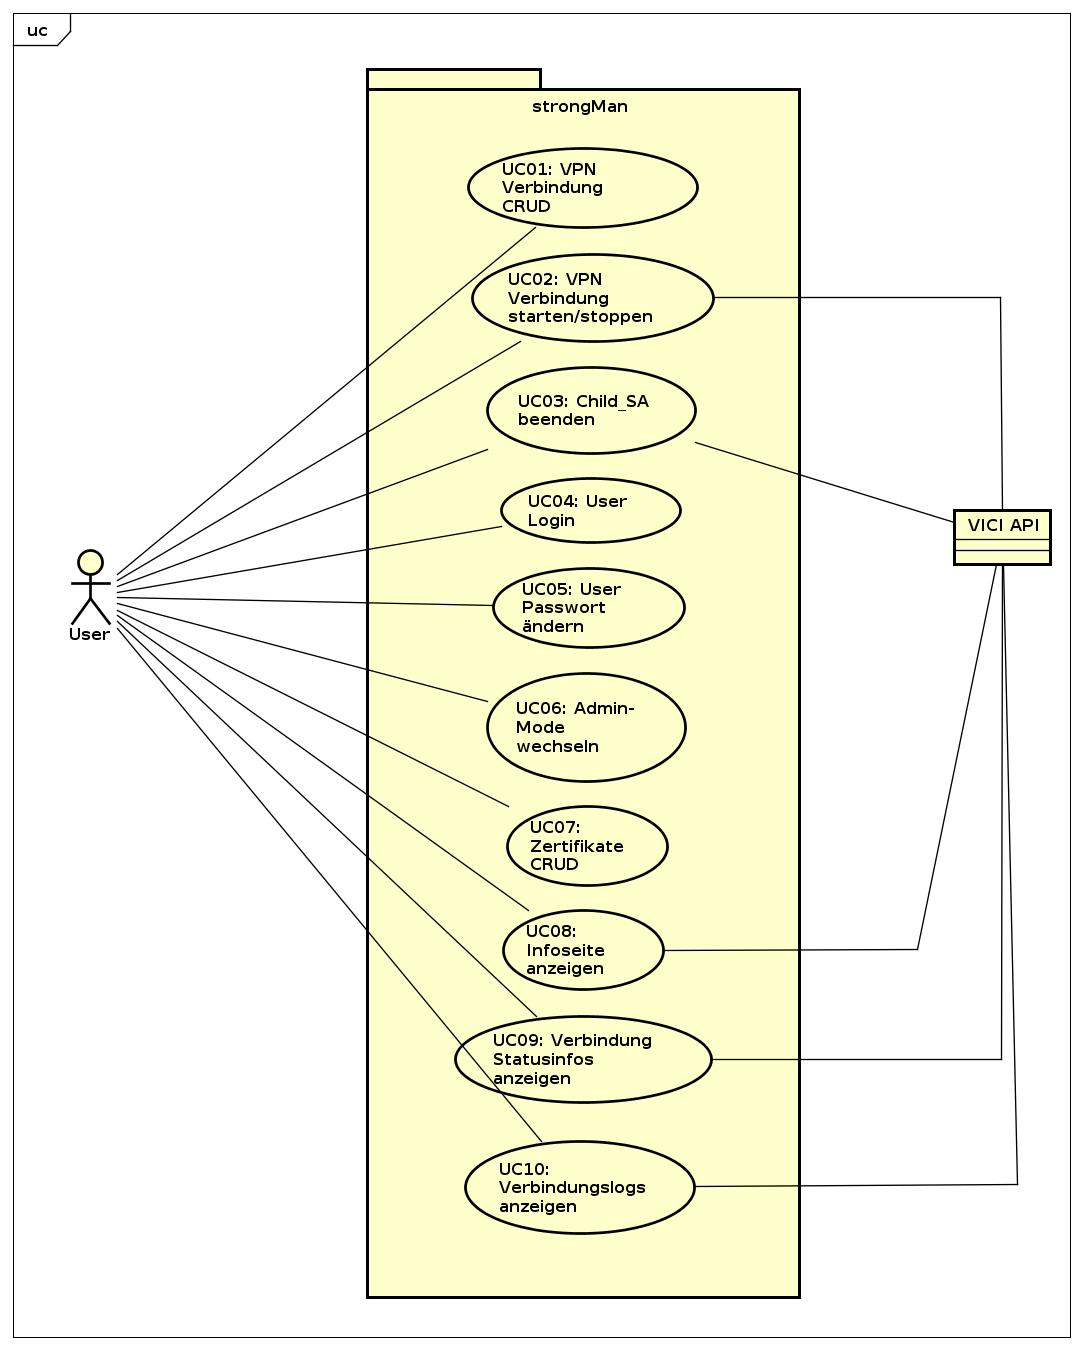
\includegraphics[width=370pt]{images/usecases.jpg}
\caption[Use Case Diagramm]{Use Case Diagramm}
\end{figure}


\subsubsection{Use Cases Brief}
Alle hier definierten Use Cases haben auch ein entsprechendes Mockup im Anhang.
\paragraph{UC01: VPN-Verbindung CRUD}\mbox{} \\
Der User kann eine VPN-Verbindung erfassen / konfigurieren. Dabei hat er eine Auswahl von verschiedenen vordefinierten Verbindungstypen. Jeder Verbindungstyp hat vordefinierte Konfigurationsfelder, die der User ausfüllen muss. Die Verbindungs-Übersichtsseite stellt die Hauptseite der Applikation dar. Dort können die Verbindungen bearbeitet und gelöscht werden.

\paragraph{UC02: VPN-Verbindung starten/stoppen}\mbox{} \\
Der User kann eine erfasste VPN-Verbindung starten und stoppen. Dabei wird die Konfiguration über die VICI-Schnittstelle geladen. Falls eine VPN-Verbindung nicht aufgebaut werden kann, soll eine passende Fehlermeldung angezeigt werden. 

\paragraph{UC03: Child\_SA beenden}\mbox{} \\
Jeder VPN-Verbindung kann mehrere Child\_SA aufbauen. Diese werden in der Hauptseite angezeigt und können vom User beendet werden. Auch dieser Use Case interagiert mit der VICI-Schnittstelle. Nur im Server Modus.

\paragraph{UC04: User Login}\mbox{} \\
Der User loggt sich zu Beginn des Webseiten Aufrufs mit einem Usernamen und Passwort ein. Es existiert nur ein Benutzer.

\paragraph{UC05: User Passwort ändern}\mbox{} \\
Sobald der User eingeloggt ist, hat er die Möglichkeit, sein Passwort zu ändern. Dabei gibt er sein altes Passwort einmal und sein neues Passwort zweimal an.

\paragraph{UC06: Admin-Mode wechseln}\mbox{} \\
\textbf{Optional:} Das Userinterface unterscheidet zwischen zwei Modis: User- und Admin-Mode. Der Modus soll über das Userinterface wechselbar sein. Der Admin-Mode stellt einige Server-spezifische Funktionalitäten zusätzlich zur Verfügung, welche der User zur einfacheren Bedienung nicht sieht.

\paragraph{UC07: Zertifikate CRUD}\mbox{} \\
Dem User wird eine Zertifikatsverwaltung zur Verfügung gestellt. Er kann Zertifikate und private Schlüssel in den gängigen Formaten uploaden, anschauen und wieder löschen. Die Dateien können mit einem Passwort verschlüsselt sein. 

\paragraph{UC08: Infoseite anzeigen}\mbox{} \\
Die Informationsseite zeigt dem eingeloggten User verschieden Informationen des strongSwans zum Beispiel Version, installierte Plugins usw.

\paragraph{UC09: Verbindung Statusinfos anzeigen}\mbox{} \\
Die Statusinformationen zu einer Verbindung zeigt dem User Traffic Selektoren und den Input/Output Traffic.

\paragraph{UC10: Verbindungslogs anzeigen}\mbox{} \\
Zeigt die Loginformationen an, die beim Verbindungsauf- und abbau von strongSwan empfangen werden.

\newpage




